\documentclass{llncs}
\usepackage{graphicx}
\usepackage{url}
\usepackage{subfigure}
\usepackage{listings}
\usepackage{color}
\usepackage{floatflt,graphicx}
\usepackage{epsfig}
\usepackage{amssymb}
\usepackage{amsmath}
\usepackage{amsfonts}
\usepackage{algorithmic}
\usepackage{paralist}
\usepackage{alltt} %Verbatim extended
\usepackage{pifont}

%%%%%%%%%%%%%%%%%%%%%%%%%%%%%%%%%%%%%%%%%%%%%%%%%%%%%%%%%%%%%%%%%%%%%%%%%%%%%%%%%%%%%%%%%%%
%% ISWC SWUI Position Paper
%% See http://swui.webscience.org/SWUI2009

\definecolor{lightblue}{rgb}{.3,.5,1}
\definecolor{orange}{rgb}{1,.7,0}
\definecolor{darkorange}{rgb}{1,.4,0}
\definecolor{darkgreen}{rgb}{0,.4,0}
\definecolor{darkblue}{rgb}{0,0,.4}
\definecolor{darkred}{rgb}{.56,0,0}
\definecolor{gray}{rgb}{.2,.2,.2}
\definecolor{shadecolor}{gray}{0.7}

\lstset{
      basicstyle = \scriptsize \ttfamily,%
      keywordstyle = [1]\color{darkgreen},%
      stringstyle  = \ttfamily\color{darkred},%
      commentstyle = \itshape\color{darkblue},%
      showstringspaces = false,%
%     fancyvrb = true,%
      firstnumber = auto, stepnumber=1, numbersep=5pt,%
      numbers=left, numberstyle=\tiny \ttfamily,
      frame = shadowbox, frameround = ffff, rulesepcolor = \color{shadecolor},
      breaklines=true, breakatwhitespace=true,%
%     prebreak=\textellipsis,postbreak=\textellipsis,%
      emphstyle = \color{red}\underbar, emphstyle = {[2]\color{blue}\underbar},%
      extendedchars = true, inputencoding = utf8,%
%     backgroundcolor=\color{shadecolor},
      xleftmargin=20pt, xrightmargin=10pt,
      captionpos = b
}


%% define N3 look and feel
\lstdefinelanguage{N3}{
      morekeywords=[1]{@prefix, a },
      morestring=[b]",
      morecomment=[s]{<}{>}, % misusing comments for URIrefs
      otherkeywords={^, [, ], (, )},%
      %otherkeywords=[2]{<, >},% for URIrefs
      sensitive=false%
}[keywords,comments,strings]

\lstset{
      basicstyle = \scriptsize \ttfamily,%
      keywordstyle = [1]\bfseries\color{darkgreen},%
      stringstyle  = \ttfamily\color{darkred},%
      commentstyle = \itshape\color{darkblue},%
      showstringspaces = false,%
%     fancyvrb = true,%
      firstnumber = auto, stepnumber=1, numbersep=5pt,%
      numbers=left, numberstyle=\tiny \ttfamily,
      frame = shadowbox, frameround = ffff, rulesepcolor = \color{shadecolor},
      breaklines=true, breakatwhitespace=true,%
%      prebreak=\textellipsis,postbreak=\textellipsis,%
      emphstyle = \color{red}\underbar, emphstyle = {[2]\color{blue}\underbar},%
      extendedchars = true, inputencoding = utf8,%
%     backgroundcolor=\color{shadecolor},
      xleftmargin=5pt, xrightmargin=2pt,
      captionpos = b
}

\begin{document}

\title{Constrained Natural Language Parser for Semantic Web Based Policies}

\author{Oshani Seneviratne \and Eunsuk Kang \and Harshad Kasture}

\institute{MIT CSAIL, Cambridge\\
Massachusetts, USA\\ 
\email{( oshani | eskang | harshad )@csail.mit.edu }
}

\maketitle
\begin{abstract}

We propose the Policy Parser, a system for translating
policies and rules in a natural language into an equivalent RDF
representation. The Policy Parser uses templates to convert informal
but structurally-constrained sentences into machine-readable
policies, which are expressed in the Accountability In RDF (AIR)
policy language. A sentence is parsed using a feature-based
context-free grammar, which extracts semantic information from the
sentence to build a corresponding parse tree. The information
contained in the parse tree is then processed to build an AIR
policy. AIR policies are represented as Turtle statements and can be
used to express security and privacy constraints in a variety of
ontologies. We present a Firefox sidebar extension as the user
interface for this system. We believe that it provides a natural
interface for authoring policies in RDF.

\end{abstract}

%%%%%%%%%%%%%%%%%%%%%%%%%%%%%%%%%%%%%%%%%%%%%%%%%%%%%%%%%%%%%%%%%%%%%%%
%% Introduction

\section{Introduction}								
\label{sec:intro}

The growth in the sheer volume and variety of information on the web
shows no signs of slowing down, and electronic information systems are
attracting a wider range of users than ever. Administrators of these
systems face a challenging task: determining and enforcing policies
for controlling the access of information. 

Unfortunately, many of the existing systems do not posess the
capacity to keep up with the rapid expansion of the data set and the
user base. The functionality for policy enforcement is often built
into a system during its initial development. As a result, access
control in most of these systems is rather limited and inflexible to changes.
As a need for new policies arises or usage scenarios grow
more complex, the administrator may need to modify parts of the system
that are responsible for maintaining and enforcing the policies. This
can be a costly and error-prone process. 

Furthermore, the creator and the maintainer of the policy may be
different from the original developer of the system. Therefore, the
system must also provide a mechanism for transforming policies, 
which are often incepted as natural language sentences, into a precise
form that can be understood by the enforcement module.

We propose a potential solution to these challenges. Our prototype
system, called the Policy Parser, consists of two major parts:
(1) a graphical front-end, which translates an input natural language policy
into a set of RDF tuples, and (2) the Accountability In RDF (AIR)
reasoner, which automatically carries a series of logical
deductions to check whether a policy is enforced by a particular usage
scenario. The front-end uses templates to capture and extract
essential components of a policy and translate them into RDF tuples;
it can be easily extended with additional templates as the types of
policies diversify. Many forms of policy enforcement are
reducible to the logical reasoning that can be performed by the AIR
reasoner. Thus, even when policies undergo changes, the
underlying enforcement engine in our system need not be modified.

%Lawyers work with laws and policies all the time. They also determine given a scenario and a set of policies, whether a particular sequence of events in this scenario violates one or more of the given policies. Enforcing policies can be a challenging and error-prone process, as the number of policies gets larger or the scenario itself becomes more complex. In some cases, for example enforcing privacy policies governing access to data on the World Wide Web, manual enforcement of policies is particularly inefficient. Fortunately, some parts of the policy enforcement process are purely deductive reasoning, and therefore, can be automated by a computer. 

%The AIR reasoner\cite{air} takes input policies and scenarios expressed in RDF and determines whether or not the given scenario violates any of the given policies. One of the current barriers to wide spread use of AIR, or any other semantic web policy language is that it requires the user (person who specifies the policies; often a lawyer) of the system to write the AIR policies in RDF. Although RDF is a well-known within the Semantic Web community, it is likely that most lawyers will not be well versed in its use. Even for someone who is an expert in RDF, translating a natural language policy into RDF can be tedious and a time-consuming task. It thus becomes difficult to create and update policies that can be enforced automatically.

%As a first step towards addressing these challenges, we have built the Policy Parser, which takes a policy, written in constrained natural language, and automatically translates it into its RDF representation.

This paper is organized as follows:
Section \ref{background} gives the overview of the technologies used and AIR policy language.  
Section \ref{design} gives a comprehensive description of the overall design and implementation of the system.
Section \ref{related} discusses the related work in this area.
Finally, we conclude the paper with a summary of the contributions and some future work in section \ref{conclusion}.


%%%%%%%%%%%%%%%%%%%%%%%%%%%%%%%%%%%%%%%%%%%%%%%%%%%%%%%%%%%%%%%%%%%%%%%
%% Background

\section{Background} \label{background}


%%%%%%%%%%%%%%%%%%%%%%%%%%%%%%%%%%%%%%%%%%%%%%%%%%%%%%%%%%%%%%%%%%%%%%%
%% Design and Implementation

\section{Design and Implementation} \label{design}

Figure \ref{fig-architecture} gives the design of the Policy Parser.

The user enters a policy sentence into our system which is a Firefox sidebar extension available here (Step 1). The sentence is then parsed using a feature-based context-free grammar (FCFG) which extracts semantic information of interest from the input natural language policy. This parsing system is built on top of the NLTK system [2] and the feature parsing library (featureparse) [3]. The semantic information contained in the natural language sentence is recorded in the features of the parse tree. In Step 3, the Policy Interpreter then further processes and analyzes this semantic information about the policy (e.g. the actor who is responsible for a particular action) contained in the features of the parse tree and bundles it up into a suitable form, which is then passed to the RDF Generator. The RDF generator generates an RDF file that corresponds to this policy and stores it in a persistent location (URI) on the web (Steps 4 and 5). The user can immediately (or at any later convenient time) check the compliance/violation of the policy by providing the URI and a particular scenario to the AIR reasoner (Steps 6 - 8), which is executible directly from the web.

\begin{figure}[!h]
  \centerline{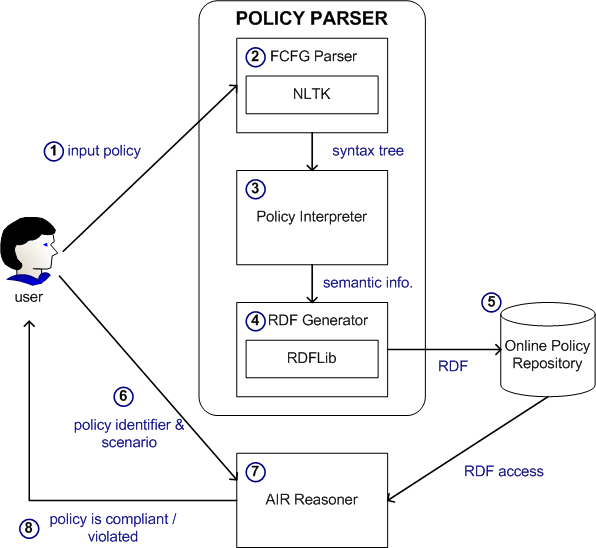
\epsfig{file=images/architecture.png, , height=4in}}
  \caption{Architecture of the Policy Parser}
  \label{fig-architecture}
\end{figure}

%% NLTK Parser

\subsection{NLTK Parser}

Given a user's input policy, the first step is to parse this sentence into a structured format that can be manipulated further by a computer. As stated earlier, we do this using FCFGs. Each of the constituents of a policy statement (subject, action etc.) are further composed of simpler constituents such as noun phrases (NPs), verb phrases (VPs) etc. The permissible forms for each constituent as well as its sub-parts, and the relation of a node's semantic value with that of its children is specified by the FCFG. The start node of the FCFG (S) has a feature corresponding to each of the constituents (subject, action etc.) mentioned above. Since we are interested in the semantic interpretation of the natural language policy, we use the sem feature to record semantic values and propagate them up the parse tree by combining the semantic values of a node's children. The values of features like subject, action, object etc. are derived from the values of the sem features of various constituents. Since we assume a rather constrained form of input, we are able to develop a simple grammar that parses sentences of the form described above and is able to infer the semantic role of a word in the sentences from its position in the parse tree relative to other constituents. In particular, we don't have to worry about many complications that arise in unconstrained natural language with quantifiers.

The words recognized by the system and their categories (N,V etc.) are included in a lexicon file. Spelling changes for words in the lexicon are handled by a kimmo rule (yaml) file. We have thus modularized our implementation so that the feature-based CFG is decoupled from the lexicon and the spelling rule changes. Also, the lexicon and the spelling change rules allow us to do some clever things, for example, the two sentence snippets ``...for criminal investigation..." and ``...to investigate crime..." lead to the same value for the feature purpose (purpose = (investigate crime)). This gives the user of the system some freedom in expressing a policy. This is particularly important in light of the way the AIR policy associates sentence fragments with predefined ontologies (as explained in the section on the RDF Generator). This and other such techniques may be used to make the system more flexible.

For example, the sentence above, ``Police may search people's homes for criminal investigation if the police have a warrant" is parsed into the syntax tree given in Figure \ref{fig-syntax-tree}.

@@TODO: Remove this parse tree? barely legible

\begin{figure}[!h]
  \centerline{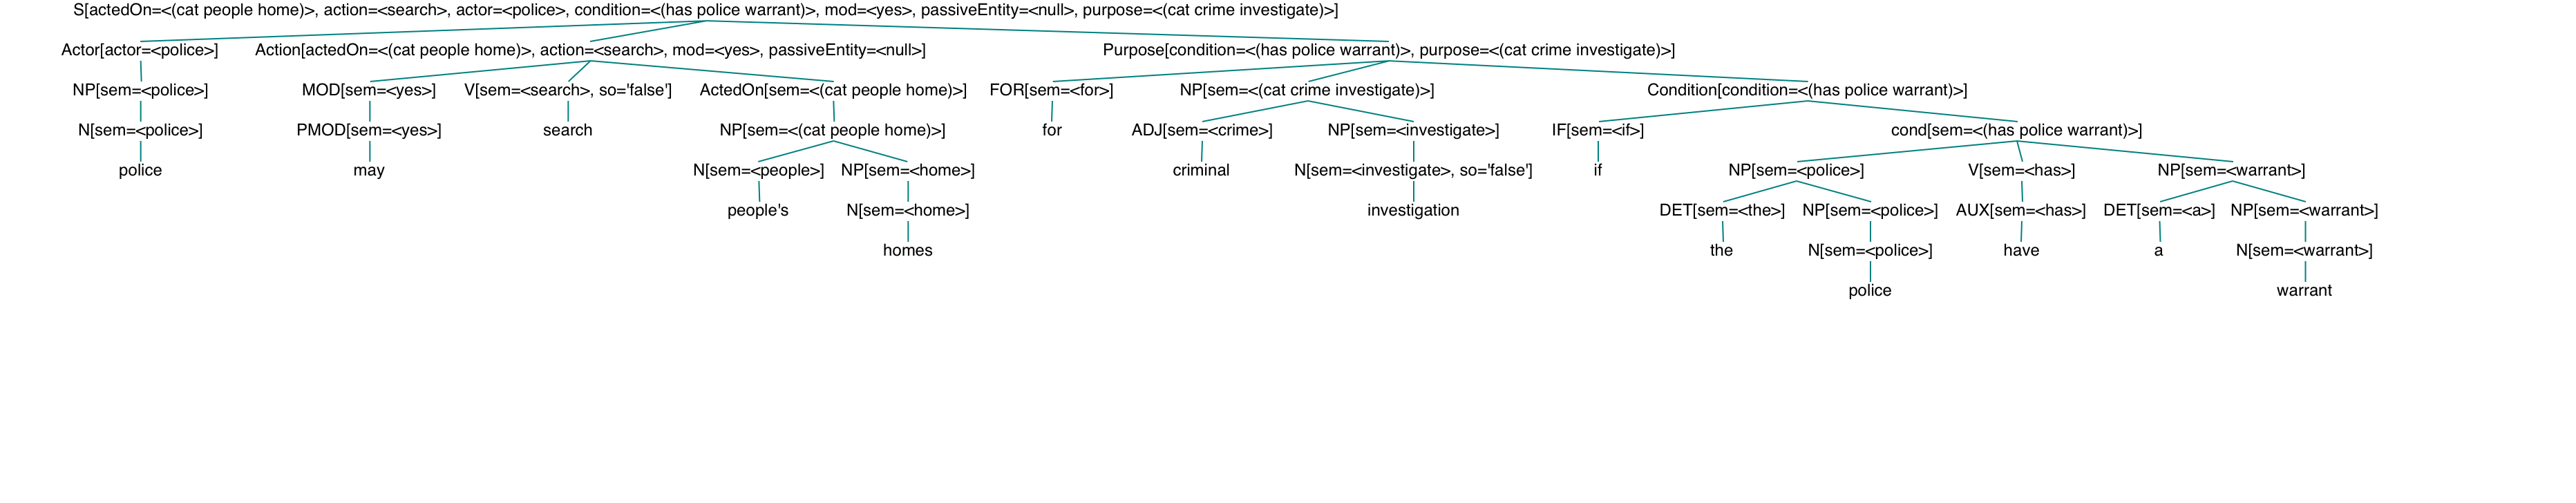
\epsfig{file=images/example_parse_tree.png, width=9in}}
  \caption{An example parse tree}
  \label{fig-syntax-tree}
\end{figure}

As shown in the syntax tree, the left-hand side of the top-level production rule `S' contains a feature for each of the semantic constituents (for example, the feature ``action" for the action constituent in the policy) for the natural language rule. The value assigned to each top-level feature is defined in terms of features from the subtrees. Note that the l.h.s. of each part-of-speech rule (e.g. `NP' for noun-phrase) is augmented with the `sem' feature; this allows us to assign a logical expression to each node in the tree. Here, we use the application of the lambda function `cat' to concatenate one or more lexicons into a single constituent.

By explicitly defining a top-level feature corresponding to each constituent of interest, the implementation of the Policy Interpreter (the next component in the pipeline) is greatly simplified - it just needs to walk over the list of top-level features and map each to a corresponding RDF construct.

We make us of the existing infrastructure in the Natural Language Toolkit (NLTK) \cite{nltk} for this part of the Policy Parser. More specifically, we use the featureparser class, which in turn is built on top of the Natural Language Toolkit for Python. In addition to a user's sentence, the FCFG parser in NLTK requires three arguments; the FCFG grammar (stored as a .fcfg file), the spelling change rules (a Kimmo file), and the lexicon (.lex file). 

%% Policy Interpreter

\subsection{Policy Interpreter}

Given a syntax tree generated by the NLTK Parser, the role of the Policy Interpreter is to extract the semantic information about the user's policy - i.e. the value for each of the constituents in the policy. As mentioned above, this process is relatively straightforward, as it simply involves looking through the list of features that are stored in the root of the syntax tree. The only intricate step in this process is walking over a lambda-calculus expression that is a concatenation of multiple lexical tokens (e.g. `(cat prox (cat card data))' for ``prox card data"); this step is implemented using a recursive function for traversing an expression.

The output from the Policy Interpreter is a dictionary (i.e. a list of key-value pairs) that maps each constituent to its value. For example, given the syntax tree for the sentence ``Committee on Discipline may access prox card data for criminal investigation", the Policy Interpreter outputs the following dictionary:

\begin{table}[h]
\centering
\begin{tabular}{|c|c|}
\hline
\textbf{Key} & \textbf{Value}\\
\hline
POLICY & MIT Prox Card Policy (\verb!name of the policy! )\\
ENTITY & Committee on Discipline (\verb!actor!)\\
FLAG & True (\verb!modality - True for positive, such as 'can' ! )\\
ACTION & use \\
PURPOSE &investigate crime \\
DATA & prox card data (\verb!object!) \\
CONDITION  &[  ] \\
SECONDARY ENTITY & None\\
\hline
\end{tabular}
\caption{Example Policy Interpreter Output}
\label{tab:policy-interpreter-output}
\end{table}

Note that some of the keys in the dictionary have different names than the constituents, but there is a 1-1 correspondence between these two sets of names. The renaming was done due to the fact that RDF uses a set of pre-designated identifiers for its constructs. 

%% RDF Generator

\subsection{RDF Generator}

This module is responsible for generating AIR \cite{air} policies. Once the user's sentence is fragmented into the relevant constituents as described above, it will identify the corresponding RDF segments and create the RDF graph using the RDFLib \cite{rdflib} Python library.

AIR is a rule-based policy language written in RDF for accountability and access control. Each AIR policy consists of one or more rules:

\begin{verbatim}
policy = { rule* } 
\end{verbatim}

Each rule is made up of a pattern that when matched causes an action to be fired. Optionally there could be description and justification elements as well.

\begin{verbatim}
rule = { pattern, action [ description justification ] } 
\end{verbatim}

An action can either be an assertion (which is a set of facts that are added to the knowledge base) or a nested rule.

\begin{verbatim}
action = { assertion | rule } 
\end{verbatim}

The basic skeleton of an AIR policy is as follows:

\begin{verbatim}
:SomePolicy a air:Policy;
air:rule [
	air:variable { ... };
	air:pattern { ... };
	air:assertion { ... };
	air:rule [ ... ]
	].
\end{verbatim}
	 		
In order to generate an AIR policy from a constrained natural language sentence, two additional parameters, besides the policy itself, are required: (1) Name for the policy (2) One or more domain ontologies. The name of the policy is required because the user should be able to identify the policy, and it is not suitable to have a random machine-generated policy name. The domain ontology is required because some of the sentence fragments need to be identified with the corresponding term (which could be either a subject or a predicate or an object) in RDF.

The Figure \ref{fig-rdf-gen} shows how the dictionary keys and values from the Policy Interpreter is used in constructing the AIR policy.

\begin{figure}[!h]
  \centerline{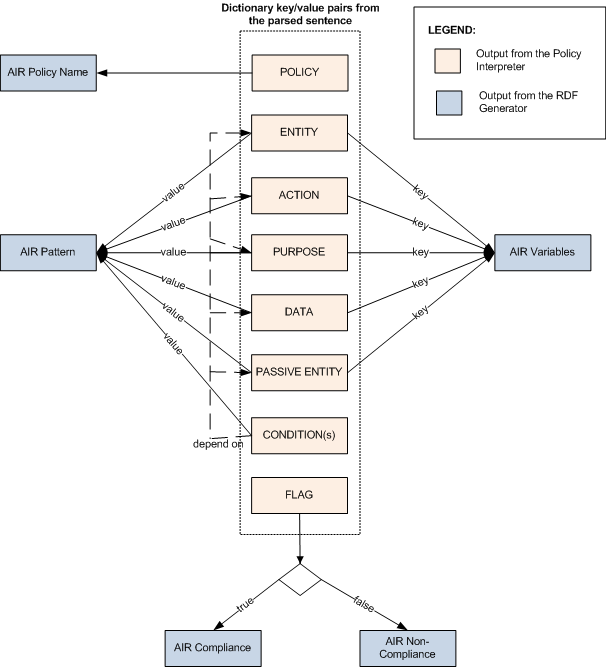
\epsfig{file=images/rdf_gen.png, height=4in}}
  \caption{The process of generating RDF from the parse tree}
  \label{fig-rdf-gen}
\end{figure}

The dictionary element 'POLICY' is used to name the policy. If the keys of dictionary elements: 'ENTITY', 'ACTION', 'PURPOSE', 'DATA' and 'PASSIVE ENTITY' have non-null values, they are used to assign air:variables. The values of these dictionary elements are then mapped on to air:patterns where each air:variables in the previous step are assigned the corresponding rdf:types.

The sentence could include conditions as in the following sentence: ``Committee on Discipline can use prox card data if the Committee on Discipline has authorization". The conditional phrase beginning with the word "if" may refer to components which are already identified, such as ``Committee on Discipline" (identified as the `ENTITY'). Therefore another pattern will be constructed with the subject, predicate or object values encoded in the `CONDITION'.

All of these steps requires proper identification of the RDF terms as defined in the ontology. SPARQL queries are used to identify the correct term from the RDF ontolgy. There is an underlying assumption that for each rdfs:Class and rdfs:Property, which corresponds to subject/object and predicate respectively, the ontology author has defined a proper rdfs:label attribute. This attribute is very much likely to be used by the policy author, hence the SPARQL query is to search for the subject which matches the dictionary value.

Finally, the 'FLAG' sent by the Policy Interpreter will determine to specify whether 'ACTION' is compliant or not with the policy.

%% Policy Editor (User Interface)

\subsection{Policy Editor}

\subsubsection{Installation and Running}

We have developed a Firefox sidebar extension which lets users write a constrained natural language sentence and parse it. You can download and install it from:
http://justparseit.googlecode.com/files/PolicyParser.xpi
\footnote{This toolbar is compatible with all the Firefox version up to 3.5}

Once it is installed on Firefox you can activate it by selecting "View -> Sidebar -> Policy Parser".
The sidebar will be displayed as shown in the Figure \ref{fig-ui}.

\begin{figure}[!h]
  \centerline{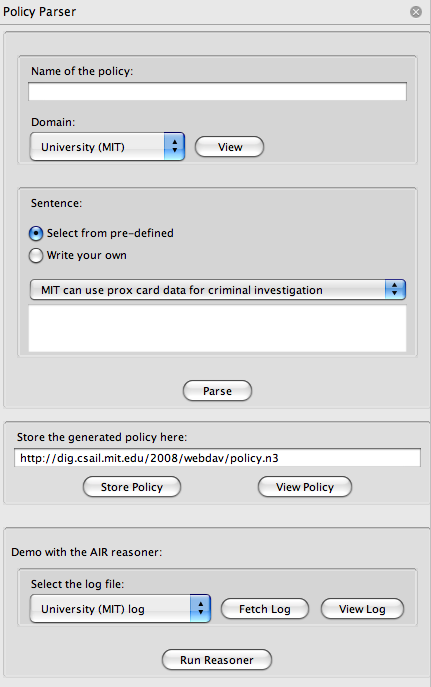
\epsfig{file=images/sidebar.png, height=3.5in}}
  \caption{User Interface of the Policy Parser}
  \label{fig-ui}
\end{figure}

First of all the user will have to specify a name for the policy that he/she intends to create. This name could be something like "MIT Prox Card Data Policy" or "Massachusetts Disability Discrimination Policy". It is up to the user to select a meaningful name.

The user will then have to select a particular domain ontology. Once the domain ontology is selected the user can view the contents of the ontology by clicking the "View" button. 
%It should be borne in mind that the lexicon of the the system is limited by the phrases indicated in the rdfs:label tags. Therefore it would be a good practice to look at the domain ontology (especially if you are writing your own sentence).

When inputing a sentence, the user has two options. He/she can select from pre-defined sentences displayed in the drop-down box (which are guaranteed to work) OR input a sentence manually by looking at the sentence format.

Once a name is given to the policy, a domain ontology is selected, and a sentence is specified, the user can press the "parse" button. This will invoke the python Policy Parser web service hosted at http://scripts.mit.edu/~oshani/justparseit/code/server/run.py with the corresponding parameters. Please note that there could be a slight delay in seeing the actual result (so please be patient!). Once the result is sent back to the browser, provided that you have installed Tabulator you would be able to see the following:

Now that you have generated the AIR policy you could make it persistant by either storing it in your local file system, or somewhere on the World Wide Web. For demonstration purposes, we have chosen to save it in a WebDAV space so that it will be universally accessible through a Universal Resource Identifier (URI). If you have your own WebDav space, please feel free to enter it in the text box underneath "Store the generated policy here: ". By default this text box contains the value:
http://dig.csail.mit.edu/2008/webdav/policy.n3. 
You could enter a new name instead of "policy.n3" and click the "Store Policy" button. When storing the policy it will ask for authorization. You can try out this feature by using the temperory username "policyparser" and password "policyparser". Once you have clicked the "Store Policy" you could view the policy in it's new storage location by clicking the "View Policy" button.

If you are interested, you can see how this generated policy may be reasoned over a log file (which includes a set of facts) by the AIR reasoner. For this particular demo, you would have to select a log file from the drop down box, and press the "Fetch Log" button. If you wish to see the contents of the log file, you have to click the "View Log" button. Once you have cicked it you should be able to see the following:

@@TODO: Give an example of a log file

If you have performed all the steps above, you are all set to invoke the AIR reasoner. Click the "Run Reasoner" button and you should be able to get the following output:

@@TODO: Give an example of the justification on the Tabulator

\subsubsection{Assumptions on User Input}

Automatically parsing an arbitrary natural language sentence is an extremely challenging task. Thus, we focus on a constrained set of natural language sentence forms. Past research has shown that constrained natural language can be effectively used for automatically generating policies, and that unconstrained natural language gives significantly poorer results \cite{karat,sparcle}. More specifically, our system assumes a specific structure for a natural language policy which is as follows:

\begin{verbatim}
subject mod action [object] [secondary_object] 
[for/to purpose] [if condition (and condition)*]
\end{verbatim}

where the meanings of the constituents are the following:

\begin{itemize}
\item \textbf{subject} The main actor or entity who carries out an action
\item \textbf{mod} The modality of the rule (i.e., whether the subject is allowed or disallowed to perform the specified action under the specified constraints, expressed using words such as "can", "cannot" etc.)
\item \textbf{action} The action performed by the subject
\item \textbf{object} The object on which the action is performed (when "action" is a transitive verb)
\item \textbf{secondary object} 
\item \textbf{purpose} An (optional) purpose for which the action is performed
\item \textbf{condition} An (optional) condition (or set of conditions) under which the rule is applicable
\end{itemize}

For example, consider the sentence "A police officer may search people's homes for a criminal investigation if the police officer has a warrant". Here, we have the following key value pairs:

\begin{itemize}
\item \textbf{subject} police officer
\item \textbf{mod} yes
\item \textbf{action} search
\item \textbf{object} people's homes
\item \textbf{secondary object} none
\item \textbf{purpose} criminal investigation
\item \textbf{condition} police officer has a warrant
\end{itemize}

Each sentence corresponds to a single policy. The constituents between '[' and ']' are optional; therefore, an input sentence must consist of, at minimum, a subject, an action and the modality of the rule. Also, '*' means "one or more"; thus, a policy may consist of any number of conditions.

%%%%%%%%%%%%%%%%%%%%%%%%%%%%%%%%%%%%%%%%%%%%%%%%%%%%%%%%%%%%%%%%%%%%%%%
%% Related Work

\section{Related Work}					\label{related}


%%%%%%%%%%%%%%%%%%%%%%%%%%%%%%%%%%%%%%%%%%%%%%%%%%%%%%%%%%%%%%%%%%%%%%%
%% Conclusion

\section{Future Work and Conclusion} \label{conclusion}

Since our underlying CFG uses spelling change automata, it can successfully parse all sentences with variations that are recognized by these automata - for example, adding ``s" to pluralize a noun or recognizing that 1st-person and 3rd-person verbs with the same root. In addition, the system (in particular the grammar and the lexicon) has been designed such that reasonable variations of a sentence give the same values for the features of interest. For example, the following two sentences result in the generation of the same AIR policies in RDF:

MIT can give records to FBI to investigate crimes.
MIT can give FBI records for criminal investigations.

Our results indicate that the system does a good job of accurately extracting semantic information from the natural language policies. It is fairly flexible in handling different forms of the input sentence. We were able to parse a variety of natural language policies into AIR policies and use them with the reasoner to check complaince of data logs. Also, while we only consider a constrained set of sentences and do not handle many interesting phenomenon (e.g. wh movement, relating pronouns to appropriate nouns in the sentence, quantifiers etc.), we believe that the system can successfully be extended to address these shortcomings. 

Three components of the system are central to the performance (generality, accuracy etc.) of the Parser . The first is the FCFG (available here), which determines the structure of sentences that the Parser is able to parse. As discussed in the Implementation page, the current FCFG recognizes the sentences of the form

\begin{verbatim}
subject [mod] action object [secondary_object] 
[for/to purpose] [if condition (and condition)*]
\end{verbatim}

The FCFG also determines the structure of each of these components and how they are assigned feature values. The FCFG can be extended to parse additional policy templates.

The second vital component is the lexicon and the spelling change rules, both of which together provide the terminals used in the FCFG. As mentioned before, this allows one to parse a wider variety of sentences by simply modifying the lexicon and/or the spelling change rules while using the same grammar. \footnote{The lexicon does not, at the moment, recognize any words with capital words: all recognized words use lower case letters only}

The third component that determines the capacity of the Policy Parser is the set of domain ontologies (combined into a single file), which act as vocabularies during RDF generation. Therefore, even if the system is able to parse (NLTK parser) and interpret (Policy Interpreter) an input policy, it cannot generate a corresponding RDF if the constituents of the policy cannot be mapped to corresponding components of an ontology. However, once all ontologies relevant to a domain (e.g. MIT prox card data access) have been defined, anyone can very easily make new rules or modify existing ones, and it is from this fact that makes such a system valuable.

All these three parameters together define the limits of what our system can do, and they can be suitably extended to make the system more flexible. For example, the FCFG can be modified to handle a wider variety of sentence structures; the lexicon can be expanded; and new ontologies can be added to generate more AIR policies.

The following is a list of Future Work we are interested in investigating further:

Support the end-term goal of a fully automated policy compliance system: The main goal of the Policy Parser is to allow a simple tool for people who are not proficient enough in authoring AIR policies in RDF. While we have achieved this goal successfully (for a limited category of sentences), more work remains in the area of generating log files automatically (these are the input scenarios that need to be checked for compliance against the policies; while this was beyond the scope of this project, it is important from the point of view of the eventual goal of which this project is a part of) and reason over them with the policies which have been generated by the system to check for policy compliance.

Support for more policy sentence templates: The current implementation handles only a handful of sentence formats which includes the components ``ENTITY", ``ACTOR", ``ACTION", ``DATA", ``PURPOSE", ``PASSIVE ENTITY" and ``CONDITION"s. However many policies will have different sentence templates which needs to be addressed in the Policy Parser. Ideally there should be an interface where a policy administrator should be able to look at the available policies and modify them or add new policy templates to the system. Also support for pronouns should be supported.

Handle more complicated grammatical constructs: In our current implementation, we ignore many difficult issues such as correctly handling quantifiers, correctly associating pronouns (``he", ``she" etc.) with the nouns used in the sentence (e.g. in the sentence ``Police may search homes if they have a warrant to do that", `they' refers to `Police' and `that' refers to `searching homes'). We also don't correctly handle some common grammatical constructs, e.g. ditransitive verbs (verbs with both a primary and a secondary object) in the `purpose' and `condition'. This can be done fairly easily, but has not been done here because of the limited time frame for this project.

Extending the lexicon: Currently the interface to the user only allows to select a particular domain ontology. However, the user should have the freedom to define an ontology and add new terms into an existing ontology. Also this requires extending the lexicon used in parsing the sentence. Also, the lexicon may be designed more carefully so that it faithfully follows the etymology of each word and allows related words to be easily associated with each other without needing to define additional ontologies (relating ``criminal" with ``crime" or ``investigation" with ``investigate", which are cases we handle, are examples of this).

Devise better strategies to handle ambiguous parses: Using context free grammars for parsing has the drawback of potentially yielding multiple parse trees for a given sentence. We handle this currently by using some heuristics in the Policy Interpreter to choose one parse. While this has given reasonably good results thus far, it is likely that we will need more sophisticated ways of handling ambiguity if we want to parse a wider variety of sentences.

Give more meaningful error messages: The user might be interested in knowing the exact point of failure when a sentence could not be parsed correctly to an AIR policy written in RDF. For example the failure could be due to the fact a particular word used in the sentence is not in the lexicon, or the sentence is written in an unknown template, or the ``features" extracted by the PolicyInterpreter is not found in the domain ontology or any combination of these. Currently there is no robust mechanism of letting the user of the point of failure. However including such a feature would be beneficial.

Show the user policies in the current ``Online Policy Store": Users may be curious as to see what policies have already been generated from the system. Thus, showing them the contents of the current ``Online Policy Store" which could be a single centralized location or strewn acorss few locations would be useful.


%%%%%%%%%%%%%%%%%%%%%%%%%%%%%%%%%%%%%%%%%%%%%%%%%%%%%%%%%%%%%%%%%%%%%%%
%% Acknowledgements

\section*{Acknowledgements}


\bibliographystyle{abbrv}
\bibliography{paper}

\end{document}
